\documentclass{beamer}

\usepackage[utf8]{inputenc}
\usepackage[T1]{fontenc}
\usepackage{booktabs}

% page numbering
\setbeamertemplate{footline}[frame number]{}
\setbeamerfont{footline}{size=\large}

% remove navigation symbols
\beamertemplatenavigationsymbolsempty

% remove caption prefix
\setbeamertemplate{caption}{\raggedright\insertcaption\par}

\title{Reproducing \textit{Colorful Image Colorization}}
\author{Timo Nicolai \and Álvaro Orgaz Expósito \and Carolina Bianchi}

\begin{document}

\begin{frame}[noframenumbering,plain]
  \titlepage
\end{frame}

% --- INTRODUCTION -------------------------------------------------------------

\begin{frame}{Introduction (I)}
  Problem statement:
    \begin{itemize}
      \item Infer colours given a grayscale image
      \item Ill-posed problem due to inherent multimodality \\
            $\rightarrow$ network should predict per-pixel colour distributions \\
            $\rightarrow$ produce \textit{plausible} colourization
    \end{itemize}

  \medskip

  \begin{figure}[!htb]
    \minipage{0.28\textwidth}
      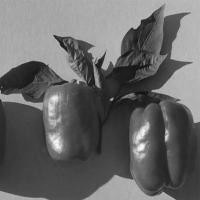
\includegraphics[width=\linewidth]{resources/bw.jpg}
      \caption{Input}
    \endminipage\hfill
    \minipage{0.28\textwidth}
      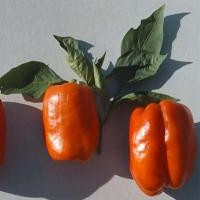
\includegraphics[width=\linewidth]{resources/gt.jpg}
      \caption{Ground truth}
    \endminipage\hfill
    \minipage{0.28\textwidth}%
      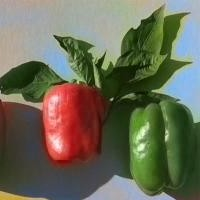
\includegraphics[width=\linewidth]{resources/colored.jpg}
      \caption{Colourized}
    \endminipage
  \end{figure}
\end{frame}

\begin{frame}{Introduction (II)}
  Applications:
    \begin{itemize}
        \item Colouring historical images.
        \item Preprocessing step in b/w image classification.
    \end{itemize}
\end{frame}

% --- RELATED WORK -------------------------------------------------------------

\begin{frame}{Related work (I)}
  Early approaches to the problem:

    \medskip

    \begin{itemize}
      \item Synthetize colours from reference pictures (Welsh et al., 2002)

      \begin{figure}[!htb]
        \minipage{0.50\textwidth}
          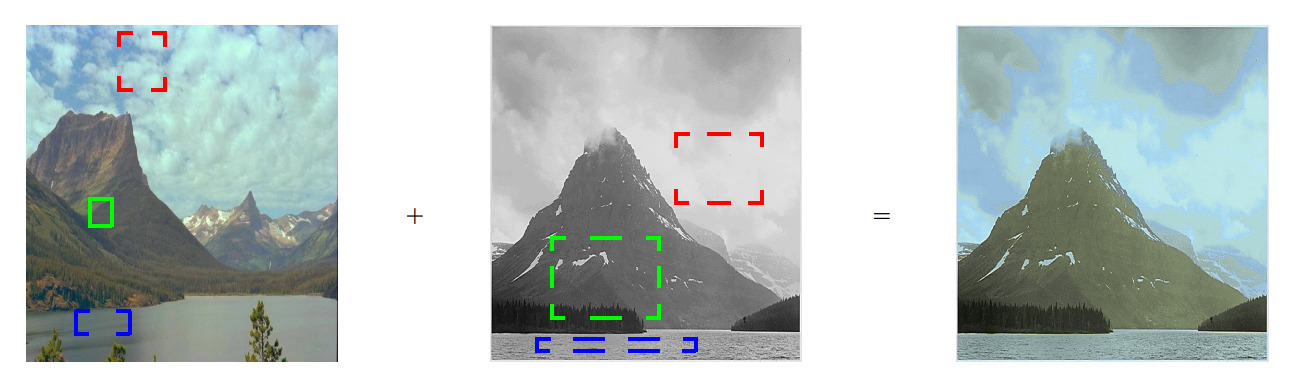
\includegraphics[width=\linewidth]{resources/welsh.jpg}
        \endminipage
      \end{figure}

      \medskip

      \item Colourization as an optimization problem (Levin et al., 2004)

      \begin{figure}[!htb]
        \minipage{0.50\textwidth}
          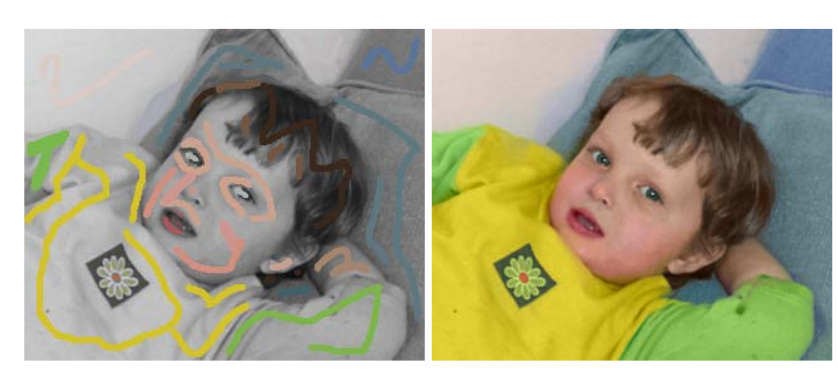
\includegraphics[width=\linewidth]{resources/levin.jpg}
        \endminipage
      \end{figure}
    \end{itemize}
\end{frame}

\begin{frame}{Related work (II)}
  Modern approaches:
    \begin{itemize}
      \item Leverage large-scale data: deep learning approaches with different
            architectures and cost functions (Larsson et al. 2016,
            Iizuka et al. 2016, \textbf{Zhang et al. 2016})
      \item Use Generative Adversarial Network to automatically learn the cost
            function (Nazeri et al. 2018)
      \item Exemplar-based colourization with automatic reference retrieval
            (He et al. 2018)
    \end{itemize}
\end{frame}

% --- DATA ---------------------------------------------------------------------

\begin{frame}{Data (I)}
  \begin{itemize}
    \item Analyze images in the L*a*b* color space \\
          $\rightarrow$ Use L channel as input \\
          $\rightarrow$ Use a and b channel as supervisory signales
    \item Resize images to 256x256 px
    \item Randomly crop images to 176x176 px during training
  \end{itemize}

  \medskip

  \begin{figure}[!htb]
    \minipage{0.24\textwidth}
      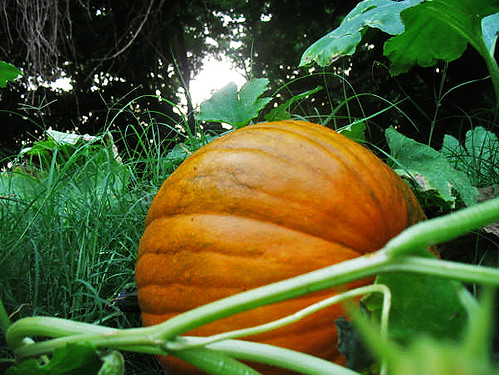
\includegraphics[width=\linewidth]{resources/pumpkin.jpg}
      \caption{Original}
    \endminipage\hfill
    \minipage{0.24\textwidth}
      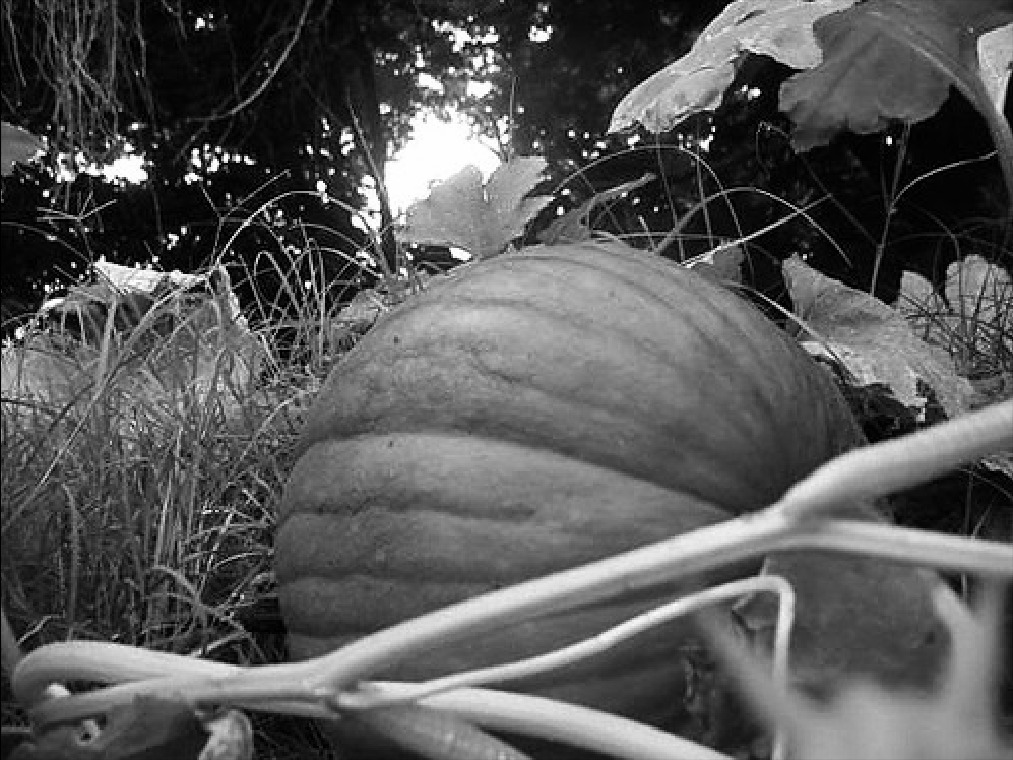
\includegraphics[width=\linewidth]{resources/pumpkin_bw.jpg}
      \caption{L channel}
    \endminipage\hfill
    \minipage{0.24\textwidth}
      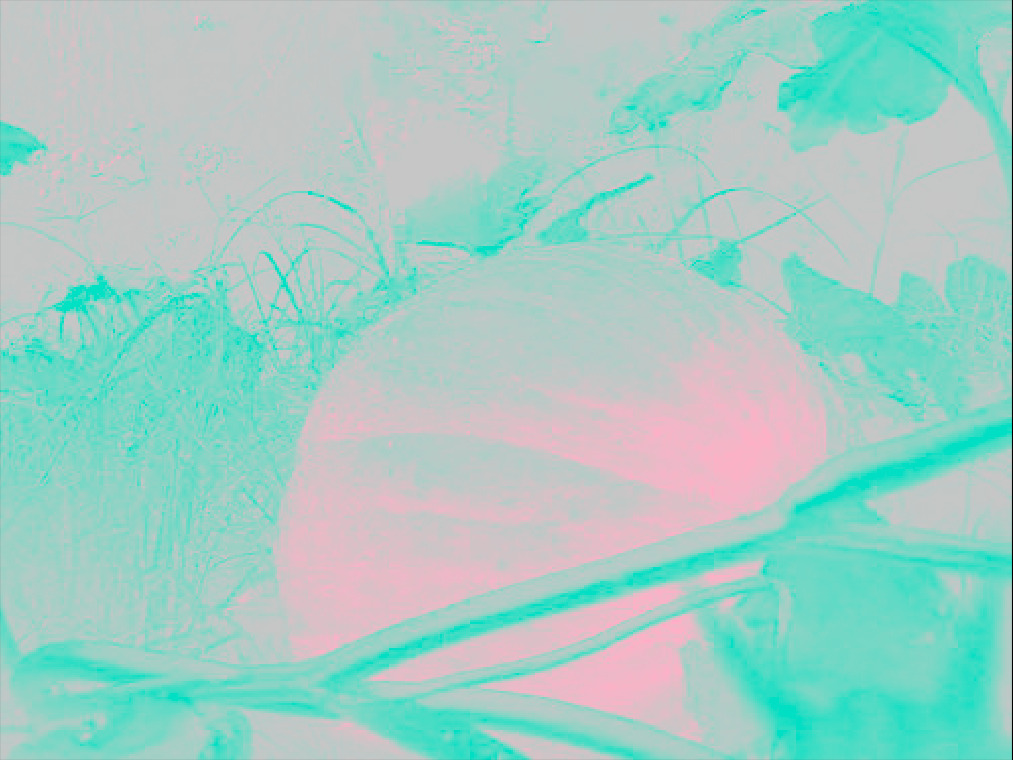
\includegraphics[width=\linewidth]{resources/pumpkin_a.jpg}
      \caption{a channel}
    \endminipage\hfill
    \minipage{0.24\textwidth}
      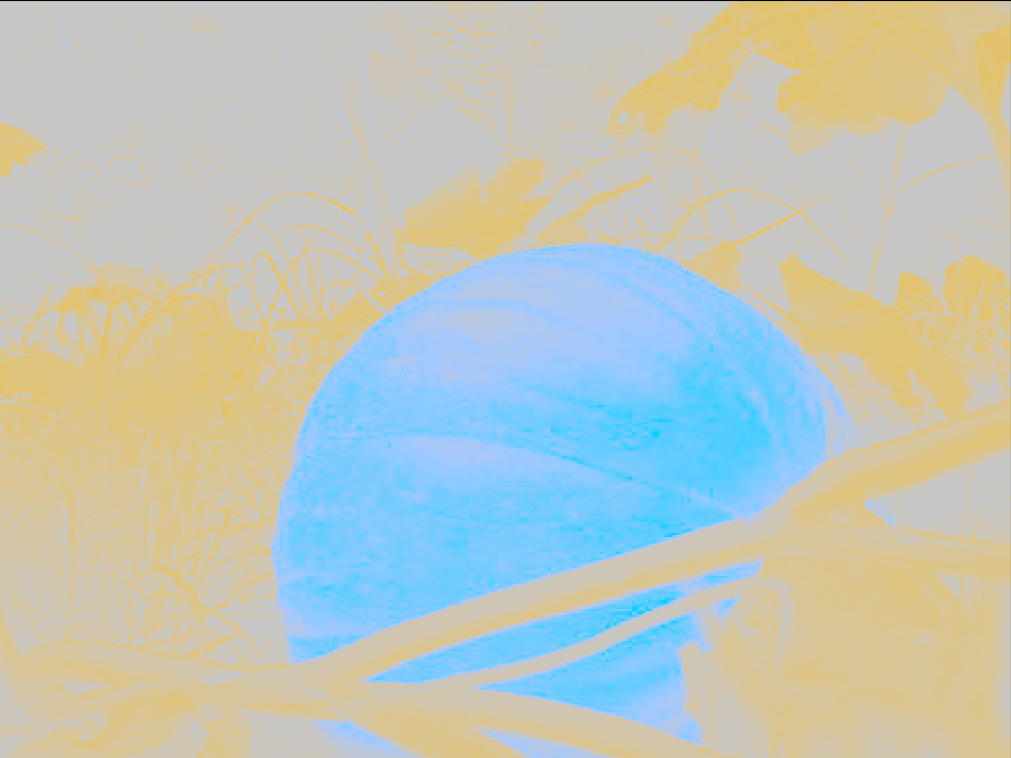
\includegraphics[width=\linewidth]{resources/pumpkin_b.jpg}
      \caption{b channel}
    \endminipage
  \end{figure}
\end{frame}

\begin{frame}{Data (II)}
  Dataset:
    \begin{itemize}
      \item Subset of ImageNet (42.566 images)
      \item Semantically related categories (mostly fruits and vegetables) \\
            $\rightarrow$ Make training feasible given computational resources \\
            $\rightarrow$ Vibrant colors: easy to inspect quality of the results
    \end{itemize}

  \medskip

  \begin{figure}
    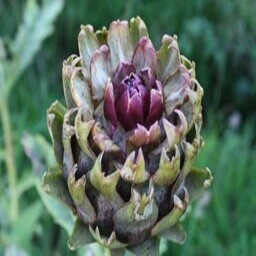
\includegraphics[width=.23\linewidth]{resources/veg1.jpg}\hfill
    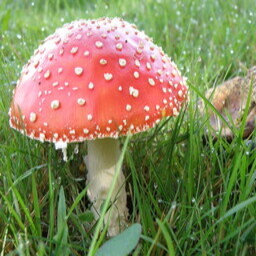
\includegraphics[width=.23\linewidth]{resources/veg2.jpg}\hfill
    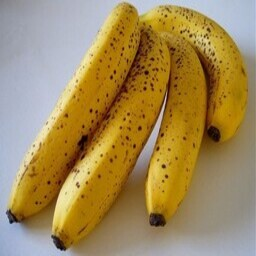
\includegraphics[width=.23\linewidth]{resources/veg3.jpg}\hfill
    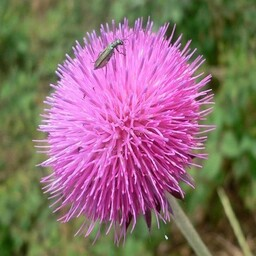
\includegraphics[width=.23\linewidth]{resources/veg4.jpg}
    \caption{Examples of images from our training set.}
  \end{figure}
\end{frame}

% --- EXPERIMENTS --------------------------------------------------------------

\begin{frame}{Training}
  \begin{center}
    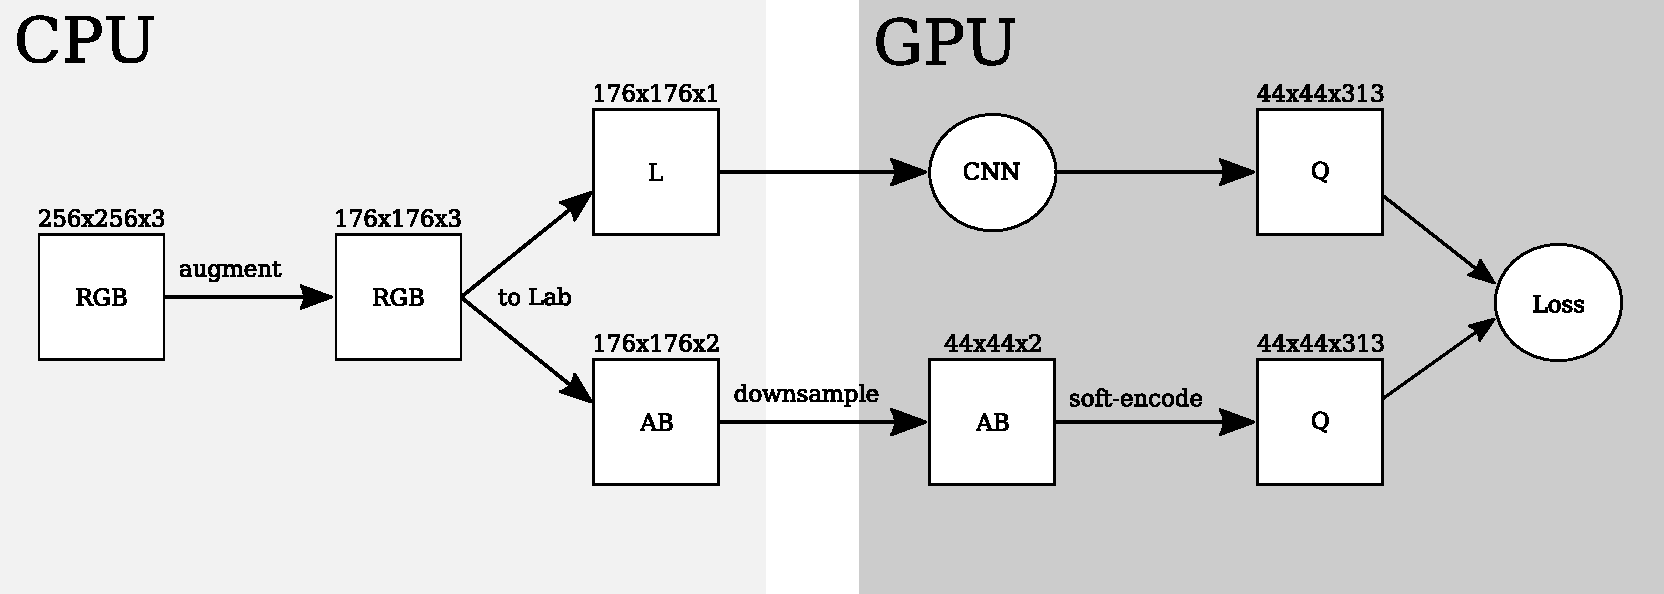
\includegraphics[width=\textwidth]{resources/training.pdf}
  \end{center}
\end{frame}

\begin{frame}{Training}
  \begin{itemize}
    \item Adam optimizer
       \begin{itemize}
         \item $\beta_1 = .9$, $\beta_2 = .99$
         \item weight decay = $10^-3$
         \item $\eta = 3.16 \time 10^{-5}$ (constant)
         \item batch size = 40
       \end{itemize}
  \end{itemize}
\end{frame}

\begin{frame}{Training}
  \begin{itemize}
    \item $\approx 20$ hours of training on NVIDIA Tesla V100
  \end{itemize}

  \begin{center}
    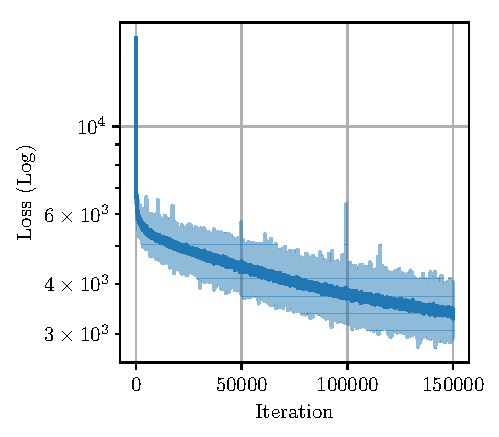
\includegraphics[width=.6\textwidth]{resources/learning_curve.pdf}
  \end{center}
\end{frame}

\begin{frame}{Examples}
  \begin{center}
    \includegraphics[height=.9\textheight]{resources/good_vs_bad_slides.pdf}
  \end{center}
\end{frame}

\begin{frame}{Perceptual Realism Study}
  \begin{center}
    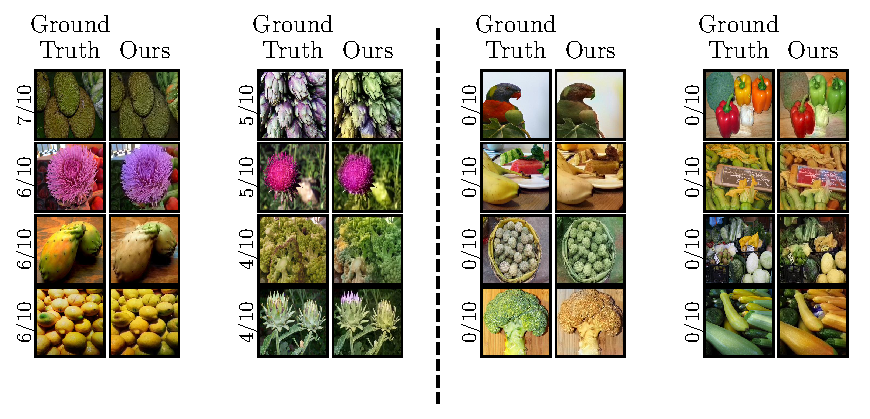
\includegraphics[width=\textwidth]{resources/amt_results_slides.pdf}
  \end{center}

  \begin{itemize}
    \item $50$ randomly chosen validation set images
    \item $10$ participants
    \item fooled on average $18.78\%$ of the time
    \item $\rightarrow$ photorealistic results only for ``easy'' images
  \end{itemize}
\end{frame}

\begin{frame}{Colourization as Preprocessing}
  \begin{center}
    \begin{tabular}{cc}
      \scalebox{0.8}{
        \begin{tabular}{ll}
          \toprule
          Method        & VGG-16 Top-5 Acc. \\
          \midrule
          Ground truth  & 92.1 \\
          Grayscale     & 46.4 \\
          Random colour & 17.4 \\
          \midrule
          Zhang et al.  & 67.7 \\
          Ours          & 81.0 \\
          \bottomrule
        \end{tabular}
      } & $\vcenter{\hbox{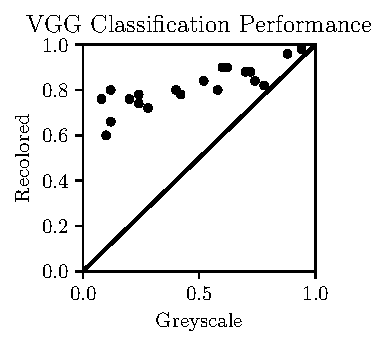
\includegraphics[width=.5\textwidth]{%
        resources/vgg_classification_performance.pdf}}}$
    \end{tabular}
  \end{center}

  \medskip

  \begin{itemize}
    \item top-5 classification accuracy for 1000 validation set images
    \item $\rightarrow$ dramatically improved by colourization!
  \end{itemize}
\end{frame}

\begin{frame}{Colourization as Preprocessing}
  \begin{columns}
    \begin{column}{0.4\textwidth}
      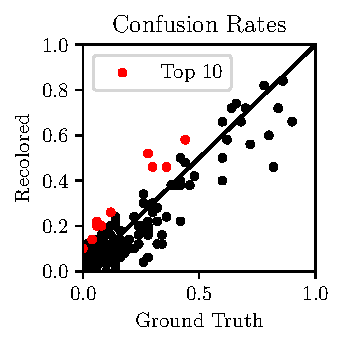
\includegraphics[width=\textwidth]{resources/confusion_rates.pdf}
    \end{column}
    \begin{column}{0.6\textwidth}
      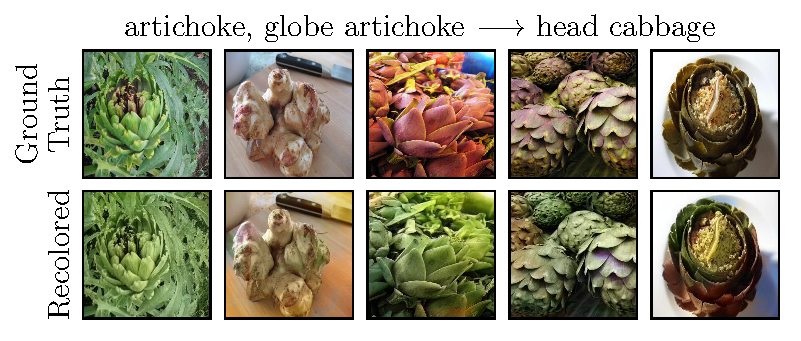
\includegraphics[width=\textwidth]{resources/common_confusions.pdf}
    \end{column}
  \end{columns}

  \medskip

  \begin{itemize}
    \item colourization amplifies certain confusion cases
  \end{itemize}
\end{frame}

\end{document}
